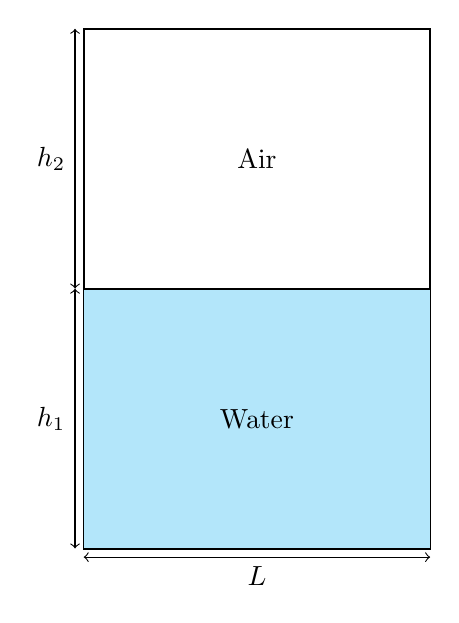
\begin{tikzpicture}[scale=1.1]

% Geometry parameters
\def\L{4}      % width
\def\Hone{3}   % water height h1
\def\Htwo{3}   % air height h2

% Outer boundary
\draw[thick] (0,0) rectangle (\L,\Hone+\Htwo);

% Water region (blue fill)
\fill[cyan!30] (0,0) rectangle (\L,\Hone);

% Interface
\draw[thick] (0,\Hone) -- (\L,\Hone);

% Phase labels
\node at (\L/2,\Hone+\Htwo/2) {Air};
\node at (\L/2,\Hone/2) {Water};


% Height h2
\draw[<->] (-0.1,\Hone) -- (-0.1,\Hone+\Htwo)
node[midway, left] {$h_2$};

% Height h1
\draw[<->] (-0.1,0) -- (-0.1,\Hone)
node[midway, left] {$h_1$};

% Width L
\draw[<->] (0,-0.1) -- (\L,-0.1)
node[midway, below] {$L$};

% % Acceleration a (horizontal)
% \draw[->] (\L+0.6,\Hone+1.2) -- (\L+1.6,\Hone+1.2)
% node[right] {$a$};

% % Gravity g (downward)
% \draw[->] (\L+1.1,\Hone+0.6) -- (\L+1.1,\Hone-0.6)
% node[midway, right] {$g$};

\end{tikzpicture}
